% Autor: Dominik Harmim <harmim6@gmail.com>

\documentclass[a4paper, 11pt]{article}

\usepackage[czech]{babel}
\usepackage[utf8]{inputenc}
\usepackage[T1]{fontenc}
\usepackage[left=2cm, top=3cm, text={17cm, 24cm}]{geometry}
\usepackage{times}
\usepackage{graphicx}
\usepackage{float}
\usepackage{amsmath}
\usepackage{scalerel}
\usepackage{booktabs}
\usepackage{multirow}

\newcommand{\intlr}[1]{\scaleleftright[1ex]{<}{#1}{>}}
\newcommand{\intopen}[1]{\scaleleftright[1ex]{(}{#1}{)}}

\setlength\parindent{0pt}


\begin{document}
	\catcode`\-=12

	\begin{titlepage}
		\begin{center}
			
\includegraphics[width=.77 \linewidth]{img/FIT_logo.pdf}

			\vspace{\stretch{.382}}

			\Huge{\textbf{Projekt z~MSP}} \\
			\LARGE{Čísla zadání: 24, 6} \\
			\Large{Cvičení\,--\,skupina: středa, 8:00}

			\vspace{\stretch{.618}}
		\end{center}

		\begin{minipage}{.47 \textwidth}
			\Large
			Datum: \today
		\end{minipage}
%
		\hfill
%
		\begin{minipage}[r]{.49 \textwidth}
			\Large
			Zpracoval: Dominik Harmim (xharmi00)
		\end{minipage}
	\end{titlepage}


	\section{
		Při kontrole výrobků byla sledována odchylka~$ X $~[mm] jejich
		rozměru od požadované velikosti. Naměřené hodnoty tvoří statistický
		soubor v~listu \\ \texttt{Data\_př.1}.
	}

	\begin{table}[H]
		\begin{tabular}{r|r|r|r|}
			\multicolumn{4}{r}{\textbf{Statistický soubor}} \\[1em]
			\cline{2-2} \cline{4-4}
			1 & $ 1,38 $ & 26 & $ 0,78 $ \\ \cline{2-2} \cline{4-4}
			2 & $ 0,72 $ & 27 & $ -0,65 $ \\ \cline{2-2} \cline{4-4}
			3 & $ 0,18 $ & 28 & $ 0,39 $ \\ \cline{2-2} \cline{4-4}
			4 & $ -0,11 $ & 29 & $ 0,49 $ \\ \cline{2-2} \cline{4-4}
			5 & $ 1,05 $ & 30 & $ 0,86 $ \\ \cline{2-2} \cline{4-4}
			6 & $ 1,45 $ & 31 & $ 1,88 $ \\ \cline{2-2} \cline{4-4}
			7 & $ -0,28 $ & 32 & $ 0,47 $ \\ \cline{2-2} \cline{4-4}
			8 & $ 2,49 $ & 33 & $ 0,51 $ \\ \cline{2-2} \cline{4-4}
			9 & $ -0,54 $ & 34 & $ 0,93 $ \\ \cline{2-2} \cline{4-4}
			10 & $ 1,88 $ & 35 & $ 3,21 $ \\ \cline{2-2} \cline{4-4}
			11 & $ 2,37 $ & 36 & $ 0,60 $ \\ \cline{2-2} \cline{4-4}
			12 & $ 0,95 $ & 37 & $ 0,40 $ \\ \cline{2-2} \cline{4-4}
			13 & $ -0,55 $ & 38 & $ 1,14 $ \\ \cline{2-2} \cline{4-4}
			14 & $ 2,05 $ & 39 & $ 2,82 $ \\ \cline{2-2} \cline{4-4}
			15 & $ 1,29 $ & 40 & $ 1,07 $ \\ \cline{2-2} \cline{4-4}
			16 & $ 0,07 $ & 41 & $ 1,32 $ \\ \cline{2-2} \cline{4-4}
			17 & $ 1,59 $ & 42 & $ 0,66 $ \\ \cline{2-2} \cline{4-4}
			18 & $ -0,20 $ & 43 & $ -0,53 $ \\ \cline{2-2} \cline{4-4}
			19 & $ -0,79 $ & 44 & $ -0,76 $ \\ \cline{2-2} \cline{4-4}
			20 & $ 0,37 $ & 45 & $ 2,80 $ \\ \cline{2-2} \cline{4-4}
			21 & $ 0,95 $ & 46 & $ 0,40 $ \\ \cline{2-2} \cline{4-4}
			22 & $ 0,97 $ & 47 & $ 0,70 $ \\ \cline{2-2} \cline{4-4}
			23 & $ -2,28 $ & 48 & $ -0,68 $ \\ \cline{2-2} \cline{4-4}
			24 & $ 2,88 $ & 49 & $ 0,19 $ \\ \cline{2-2} \cline{4-4}
			25 & $ 0,78 $ & 50 & $ -0,48 $ \\ \cline{2-2} \cline{4-4}
		\end{tabular}
%
		\hspace{4em}
%
		\begin{tabular}{r|r|r|r|}
			\multicolumn{4}{r}{\textbf{Uspořádaný statistický soubor}} \\[1em]
			\cline{2-2} \cline{4-4}
			(1) & $ -2,28 $ & (26) & $ 0,72 $ \\ \cline{2-2} \cline{4-4}
			(2) & $ -0,79 $ & (27) & $ 0,78 $ \\ \cline{2-2} \cline{4-4}
			(3) & $ -0,76 $ & (28) & $ 0,78 $ \\ \cline{2-2} \cline{4-4}
			(4) & $ -0,68 $ & (29) & $ 0,86 $ \\ \cline{2-2} \cline{4-4}
			(5) & $ -0,65 $ & (30) & $ 0,93 $ \\ \cline{2-2} \cline{4-4}
			(6) & $ -0,55 $ & (31) & $ 0,95 $ \\ \cline{2-2} \cline{4-4}
			(7) & $ -0,54 $ & (32) & $ 0,95 $ \\ \cline{2-2} \cline{4-4}
			(8) & $ -0,53 $ & (33) & $ 0,97 $ \\ \cline{2-2} \cline{4-4}
			(9) & $ -0,48 $ & (34) & $ 1,05 $ \\ \cline{2-2} \cline{4-4}
			(10) & $ -0,28 $ & (35) & $ 1,07 $ \\ \cline{2-2} \cline{4-4}
			(11) & $ -0,20 $ & (36) & $ 1,14 $ \\ \cline{2-2} \cline{4-4}
			(12) & $ -0,11 $ & (37) & $ 1,29 $ \\ \cline{2-2} \cline{4-4}
			(13) & $ 0,07 $ & (38) & $ 1,32 $ \\ \cline{2-2} \cline{4-4}
			(14) & $ 0,18 $ & (39) & $ 1,38 $ \\ \cline{2-2} \cline{4-4}
			(15) & $ 0,19 $ & (40) & $ 1,45 $ \\ \cline{2-2} \cline{4-4}
			(16) & $ 0,37 $ & (41) & $ 1,59 $ \\ \cline{2-2} \cline{4-4}
			(17) & $ 0,39 $ & (42) & $ 1,88 $ \\ \cline{2-2} \cline{4-4}
			(18) & $ 0,40 $ & (43) & $ 1,88 $ \\ \cline{2-2} \cline{4-4}
			(19) & $ 0,40 $ & (44) & $ 2,05 $ \\ \cline{2-2} \cline{4-4}
			(20) & $ 0,47 $ & (45) & $ 2,37 $ \\ \cline{2-2} \cline{4-4}
			(21) & $ 0,49 $ & (46) & $ 2,49 $ \\ \cline{2-2} \cline{4-4}
			(22) & $ 0,51 $ & (47) & $ 2,80 $ \\ \cline{2-2} \cline{4-4}
			(23) & $ 0,60 $ & (48) & $ 2,82 $ \\ \cline{2-2} \cline{4-4}
			(24) & $ 0,66 $ & (49) & $ 2,88 $ \\ \cline{2-2} \cline{4-4}
			(25) & $ 0,70 $ & (50) & $ 3,21 $ \\ \cline{2-2} \cline{4-4}
		\end{tabular}
	\end{table}

	\vspace{1em}\noindent\rule{\textwidth}{.5pt}\vspace{1em}

	a) Proveďte roztřídění statistického souboru, vytvořte tabulku
	četností a~nakreslete histogramy pro relevantní četnosti
	a~relevantní kumulativní četnosti.
	\vspace{1em}

	počet prvků statistického souboru $ n = 50 $ \\
	$ x_{(1)} = \underset{i}{\mathrm{min}}\ x_i = -2,28 $ \\
	$ x_{(n)} = \underset{i}{\mathrm{max}}\ x_i = 3,21 $ \\
	variační obor: $ \intlr{x_{(1)}, x_{(n)}} = \intlr{-2,28; 3,21} $ \\
	rozpětí: $ x_{(n)} - x_{(1)} = 5,49 $ \\
	\textbf{počet tříd} $ \boldsymbol{m = 11} $ (zvoleno) \\
	délka třídy $ = \frac{x_{(n)} - x_{(1)}}{m} = 0,49909 $

	\begin{table}[H]
		\centering
		\begin{tabular}{|r|r|r|r|r|r|r|r|}
			\hline
			\multicolumn{1}{|c|}{\textbf{třída}}
			& \multicolumn{1}{c|}{$ \boldsymbol{x_i-} $}
			& \multicolumn{1}{c|}{\textbf{$ \boldsymbol{x_i+} $}}
			& \multicolumn{1}{c|}{\textbf{střed třídy}}
			& \multicolumn{1}{c|}{\textbf{kum. četnost}}
			& \multicolumn{1}{c|}{\textbf{četnost}}
			& \multicolumn{1}{c|}{\textbf{rel. četnost}}
			& \multicolumn{1}{c|}{\textbf{rel. kum. četnost}}
			\\ \hline \hline

			$ 1 $ & $ -2,2800 $ & $ -1,7809 $ & $ -2,0305 $
			& $ 1 $ & $ 1 $ & $ 0,02 $ & $ 0,02 $ \\ \hline

			$ 2 $ & $ -1,7809 $ & $ -1,2809 $ & $ -1,5309 $
			& $ 1 $ & $ 0 $ & $ 0,00 $ & $ 0,02 $ \\ \hline

			$ 3 $ & $ -1,2809 $ & $ -0,7809 $ & $ -1,0309 $
			& $ 2 $ & $ 1 $ & $ 0,02 $ & $ 0,04 $ \\ \hline

			$ 4 $ & $ -0,7809 $ & $ -0,2809 $ & $ -0,5309 $
			& $ 9 $ & $ 7 $ & $ 0,14 $ & $ 0,18 $ \\ \hline

			$ 5 $ & $ -0,2809 $ & $ 0,2191 $ & $ -0,0309 $
			& $ 15 $ & $ 6 $ & $ 0,12 $ & $ 0,30 $ \\ \hline

			$ 6 $ & $ 0,2191 $ & $ 0,7191 $ & $ 0,4691 $
			& $ 25 $ & $ 10 $ & $ 0,20 $ & $ 0,50 $ \\ \hline

			$ 7 $ & $ 0,7191 $ & $ 1,2191 $ & $ 0,9691 $
			& $ 36 $ & $ 11 $ & $ 0,22 $ & $ 0,72 $ \\ \hline

			$ 8 $ & $ 1,2191 $ & $ 1,7191 $ & $ 1,4691 $
			& $ 41 $ & $ 5 $ & $ 0,10 $ & $ 0,82 $ \\ \hline

			$ 9 $ & $ 1,7191 $ & $ 2,2191 $ & $ 1,9691 $
			& $ 44 $ & $ 3 $ & $ 0,06 $ & $ 0,88 $ \\ \hline

			$ 10 $ & $ 2,2191 $ & $ 2,7191 $ & $ 2,4691 $
			& $ 46 $ & $ 2 $ & $ 0,04 $ & $ 0,92 $ \\ \hline

			$ 11 $ & $ 2,7191 $ & $ 3,2100 $ & $ 2,9645 $
			& $ 50 $ & $ 4 $ & $ 0,08 $ & $ 1,00 $ \\ \hline
		\end{tabular}
	\end{table}

	\begin{figure}[H]
		\centering
		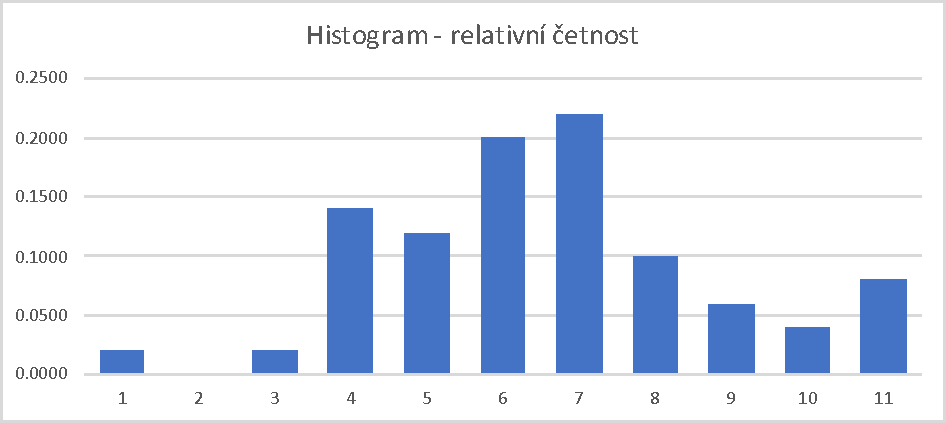
\includegraphics[width=.7 \linewidth]{img/1-a-rel-cet.pdf}
	\end{figure}

	\begin{figure}[H]
		\centering
		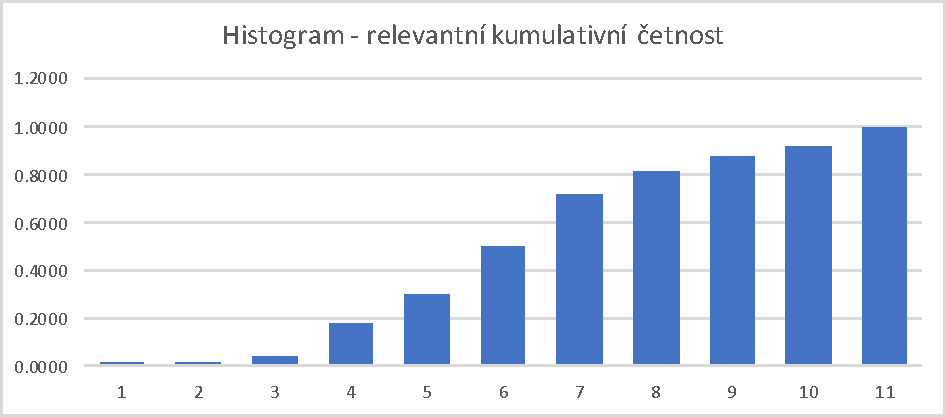
\includegraphics[width=.7 \linewidth]{img/1-a-rel-kum-cet.pdf}
	\end{figure}

	\vspace{1em}\noindent\rule{\textwidth}{.5pt}\vspace{1em}

	b) Vypočtěte aritmetický průměr, medián, modul, rozptyl a~směrodatnou
	odchylku.
	\vspace{1em}

	$ \boldsymbol{\overline{x}} = \frac{1}{n} \sum\limits_{i = 1}^n x_i =
	0,7438 $ \\
	\textbf{medián}: $ \boldsymbol{\widetilde{x}} = 0,71 $ \\
	\textbf{modus}: $ \boldsymbol{\hat{x}} = 0,4 $ \\
	$ \boldsymbol{s^2} = \frac{1}{n} \sum\limits_{i = 1}^n (x_i -
	\overline{x})^2 = 1,212 $ \\
	$ \boldsymbol{s} = \sqrt{\frac{1}{n} \sum\limits_{i = 1}^n (x_i -
	\overline{x})^2} = 1,1009 $

	\vspace{1em}\noindent\rule{\textwidth}{.5pt}\vspace{1em}

	c) Vypočtěte bodové odhady střední hodnoty, rozptylu a~směrodatné
	odchylky.
	\vspace{1em}

	\textbf{bodový odhad střední hodnoty}: $ \boldsymbol{\overline{x}} =
	\frac{1}{n} \sum\limits_{i = 1}^n x_i = 0,7438 $ \\
	\textbf{bodový odhad rozptylu}: $ \boldsymbol{s^2} = \frac{1}{n - 1}
	\sum\limits_{i = 1}^n (x_i - \overline{x})^2 = 1,2368 $ \\
	\textbf{bodový odhad směrodatné odchylky}: $ \boldsymbol{s} =
	\sqrt{\frac{1}{n - 1} \sum\limits_{i = 1}^n (x_i - \overline{x})^2} =
	1,1121 $

	\vspace{1em}\noindent\rule{\textwidth}{.5pt}\vspace{1em}

	d) Testujte předpoklad o~výběru z~normálního rozdělení Personovým
	(chí-kvadrát) testem na hladině významnosti $ 0,05 $.
	\vspace{1em}

	\begin{table}[H]
		\centering
		\begin{tabular}{|r|r|r|r|r|r|r|r|}
			\hline
			\multicolumn{1}{|c|}{\textbf{třída}}
			& \multicolumn{1}{c|}{$ \boldsymbol{x_i-} $}
			& \multicolumn{1}{c|}{\textbf{$ \boldsymbol{x_i+} $}}
			& \multicolumn{1}{c|}{\textbf{střed třídy}}
			& \multicolumn{1}{c|}{\textbf{kum. čet.}}
			& \multicolumn{1}{c|}{\textbf{četnost}}
			& \multicolumn{1}{c|}{\textbf{teor. čet.}}
			& \multicolumn{1}{c|}{$ \mathbf{rozdil^2 / teor. cet.} $}
			\\ \hline \hline

			$ 1 $ & $ -1000,0000 $ & $ -0,2809 $ & $ -500,1405 $
			& $ 9 $ & $ 9 $ & $ 8,9208 $ & $ 0,0007 $ \\ \hline

			$ 2 $ & $ -0,2809 $ & $ 0,2182 $ & $ -0,0314 $
			& $ 15 $ & $ 6 $ & $ 6,9910 $ & $ 0,1405 $ \\ \hline

			$ 3 $ & $ 0,2182 $ & $ 0,7173 $ & $ 0,4677 $
			& $ 25 $ & $ 10 $ & $ 8,6124 $ & $ 0,2236 $ \\ \hline

			$ 4 $ & $ 0,7173 $ & $ 1,2164 $ & $ 0,9668 $
			& $ 36 $ & $ 11 $ & $ 8,7036 $ & $ 0,6059 $ \\ \hline

			$ 5 $ & $ 1,2164 $ & $ 1,7155 $ & $ 1,4659 $
			& $ 41 $ & $ 5 $ & $ 7,2153 $ & $ 0,6802 $ \\ \hline

			$ 6 $ & $ 1,7155 $ & $ 1000,0000 $ & $ 500,8577 $
			& $ 50 $ & $ 9 $ & $ 9,5569 $ & $ 0,0324 $ \\ \hline
		\end{tabular}
	\end{table}

	testovací kritérium: $ t = \sum\limits_{j = 1}^m
	\frac{(f_j - \hat{f}_j)^2}{\hat{f}_j} = 1,6833 $ \\
	$ \chi_{1 - \alpha}^2 $ pro $ k = 6 - 2 - 1 $ stupňů volnosti:
	$ 7,8147 $ \\
	doplněk kritického oboru $ \overline{W}_\alpha = \intlr{0, \chi_{1 -
	\alpha}^2} = \intlr{0; 7,8147} $ \\
	Protože $ t \in \overline{W}_\alpha $, tedy hypotéza:
	$ X \sim N(0,7438; 1,1121) $ se \textbf{nezamítá}.

	\begin{figure}[H]
		\centering
		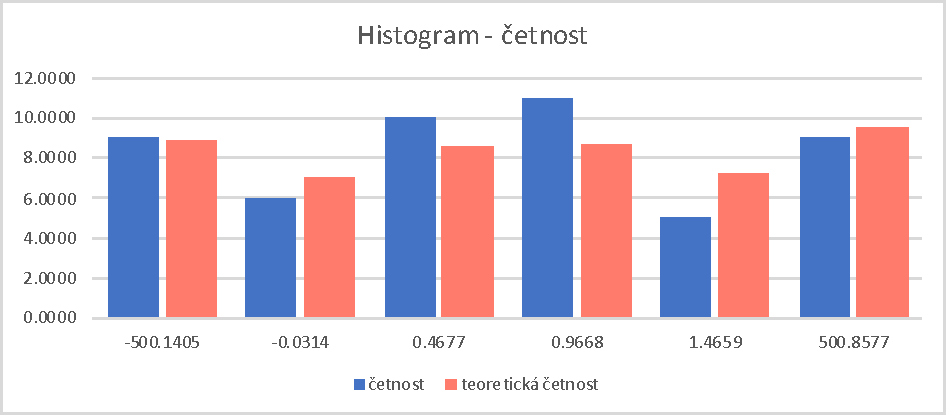
\includegraphics[width=.7 \linewidth]{img/1-d-cet.pdf}
	\end{figure}

	\vspace{1em}\noindent\rule{\textwidth}{.5pt}\vspace{1em}

	e) Za předpokladu (bez ohledu na výsledek části~d)), že statistický
	soubor byl získán náhodným výběrem z~normálního rozdělení, určete
	intervalové odhady střední hodnoty, rozptylu a~směrodatné odchylky
	se spolehlivostí~$ 0,95 $ a~$ 0,99 $.
	\vspace{1em}

	předpoklad: $ X \sim N(\mu, \sigma^2) $, $ \sigma^2 $\,--\,neznámé

	bodový odhad střední hodnoty: $ \overline{x} = \frac{1}{n}
	\sum\limits_{i = 1}^n x_i = 0,7438 $ \\
	bodový odhad rozptylu: $ s^2 = \frac{1}{n - 1} \sum\limits_{i = 1}^n
	(x_i - \overline{x})^2 = 1,2368 $ \\
	bodový odhad směrodatné odchylky: $ s = \sqrt{\frac{1}{n - 1}
	\sum\limits_{i = 1}^n (x_i - \overline{x})^2} = 1,1121 $

	\vspace{1em}
	\textbf{Intervalový odhad} parametru $ \boldsymbol{\mu} $: \\
	$ 0,975 $ kvantil Studentova rozdělení $ t_{1 - \frac{\alpha}{2}} $
	s~$ k = n - 1 = 50 - 1 = 49 $ stupni volnosti $ = 2,0096 $ \\
	$ 0,995 $ kvantil Studentova rozdělení $ t_{1 - \frac{\alpha}{2}} $
	s~$ k = n - 1 = 50 - 1 = 49 $ stupni volnosti $ = 2,68 $ \\
	$ \alpha = 0,05 $: $ \intlr{\overline{x} - t_{1 - \frac{\alpha}{2}}
	\frac{s}{\sqrt{n}}; \overline{x} + t_{1 - \frac{\alpha}{2}}
	\frac{s}{\sqrt{n}}} = \intlr{0,4277; 1,0599} $ \\
	$ \alpha = 0,01 $: $ \intlr{\overline{x} - t_{1 - \frac{\alpha}{2}}
	\frac{s}{\sqrt{n}}; \overline{x} + t_{1 - \frac{\alpha}{2}}
	\frac{s}{\sqrt{n}}} = \intlr{0,3223; 1,1653} $

	\vspace{1em}
	\textbf{Intervalový odhad} parametru $ \boldsymbol{\sigma^2} $: \\
	$ 0,975 $ kvantil Pearsonova rozdělení $ \chi_{\frac{\alpha}{2}}^2 $
	s~$ k = n - 1 = 50 - 1 = 49 $ stupni volnosti $ = 31,5549 $ \\
	$ 0,975 $ kvantil Pearsonova rozdělení $ \chi_{1 - \frac{\alpha}{2}}^2 $
	s~$ k = n - 1 = 50 - 1 = 49 $ stupni volnosti $ = 70,2224 $ \\
	$ 0,995 $ kvantil Pearsonova rozdělení $ \chi_{\frac{\alpha}{2}}^2 $
	s~$ k = n - 1 = 50 - 1 = 49 $ stupni volnosti $ = 27,2493 $ \\
	$ 0,995 $ kvantil Pearsonova rozdělení $ \chi_{1 - \frac{\alpha}{2}}^2 $
	s~$ k = n - 1 = 50 - 1 = 49 $ stupni volnosti $ = 78,2307 $ \\
	$ \alpha = 0,05 $: $ \intlr{\frac{(n - 1) s^2}{\chi_{1 -
	\frac{\alpha}{2}}^2}; \frac{(n - 1) s^2}{\chi_{\frac{\alpha}{2}}^2}} =
	\intlr{0,7760; 1,7269} $ \\
	$ \alpha = 0,01 $: $ \intlr{\frac{(n - 1) s^2}{\chi_{1 -
	\frac{\alpha}{2}}^2}; \frac{(n - 1) s^2}{\chi_{\frac{\alpha}{2}}^2}} =
	\intlr{0,6966; 1,9998} $

	\vspace{1em}
	\textbf{Intervalový odhad} parametru $ \boldsymbol{\sigma} $: \\
	$ \alpha = 0,05 $: $ \intlr{\sqrt{\frac{(n - 1) s^2}{\chi_{1 -
	\frac{\alpha}{2}}^2}; \frac{(n - 1) s^2}{\chi_{\frac{\alpha}{2}}^2}}} =
	\intlr{\sqrt{0,7760}; \sqrt{1,7269}} = \intlr{0,8809; 1,3141} $ \\
	$ \alpha = 0,01 $: $ \intlr{\sqrt{\frac{(n - 1) s^2}{\chi_{1 -
	\frac{\alpha}{2}}^2}; \frac{(n - 1) s^2}{\chi_{\frac{\alpha}{2}}^2}}} =
	\intlr{\sqrt{0,6966}; \sqrt{1,9998}} = \intlr{0,8346; 1,4141} $

	\vspace{1em}\noindent\rule{\textwidth}{.5pt}\vspace{1em}

	f) Testujte hypotézu optimálního seřízení stroje, tj. že střední
	hodnota odchylky je nulová, proti dvoustranné alternativní hypotéze,
	že střední hodnota odchylky je různá od nuly, a to na hladině
	významnosti $ 0,05 $.
	\vspace{1em}

	\textbf{Studentův jednovýběrový test:} \\
	\textbf{Testujeme hypotézu $ H_0 : \mu = 0 $ :} \\
	testovací kritérium: $ t = \frac{\overline{x} - \mu_0}{s} \sqrt{n} =
	\frac{\overline{x} - 0}{s} \sqrt{n} = 4,7293 $ \\
	doplněk kritického oboru: $ \overline{W}_\alpha = \intlr{-t_{1 -
	\frac{\alpha}{2}}, t_{1 - \frac{\alpha}{2}}} $ pro alternativní
	hypotézu: $ H_A : \mu \neq \mu_0 $ \\
	$ 0,975 $ kvantil Studentova rozdělení $ t_{1 - \frac{\alpha}{2}} $
	s~$ k = n - 1 = 50 - 1 = 49 $ stupni volnosti $ = 2,0096 $ \\
	$ \overline{W}_\alpha = \intlr{-t_{1 - \frac{\alpha}{2}}, t_{1 -
	\frac{\alpha}{2}}} = \intlr{-2,0096; 2,0096} $ \\
	Protože $ t \notin \overline{W}_\alpha $, tak hypotéza $ H_0 : \mu = 0 $
	se \textbf{zamítá} a~alternativní hypotéza $ H_A : \mu \neq 0 $ se
	nezamítá.

	\vspace{1em}\noindent\rule{\textwidth}{.5pt}\vspace{1em}

	g) Ověřte statistickým testem na hladině významnosti $ 0,05 $, zda
	seřízení stroje ovlivnilo kvalitu výroby, víte-li, že výše uvedený
	statistický soubor 50-ti hodnot vznikl spojením dvou dílčích
	statistických souborů tak, že po naměření prvních 20-ti hodnot bylo
	provedeno nové seřízení stroje a~pak bylo neměřeno zbývajících 30
	hodnot.
	\vspace{1em}

	\begin{table}[H]
		\begin{tabular}[t]{r|r|}
			\multicolumn{1}{c}{} & \multicolumn{1}{c}{$ \boldsymbol{x\ 1:20}
			$\,--\,$\boldsymbol{X} $} \\ \cline{2-2}

			1 & $ 1,38 $ \\ \cline{2-2}
			2 & $ 0,72 $ \\ \cline{2-2}
			3 & $ 0,18 $ \\ \cline{2-2}
			4 & $ -0,11 $ \\ \cline{2-2}
			5 & $ 1,05 $ \\ \cline{2-2}
			6 & $ 1,45 $ \\ \cline{2-2}
			7 & $ -0,28 $ \\ \cline{2-2}
			8 & $ 2,49 $ \\ \cline{2-2}
			9 & $ -0,54 $ \\ \cline{2-2}
			10 & $ 1,88 $ \\ \cline{2-2}
			11 & $ 2,37 $ \\ \cline{2-2}
			12 & $ 0,95 $ \\ \cline{2-2}
			13 & $ -0,55 $ \\ \cline{2-2}
			14 & $ 2,05 $ \\ \cline{2-2}
			15 & $ 1,29 $ \\ \cline{2-2}
			16 & $ 0,07 $ \\ \cline{2-2}
			17 & $ 1,59 $ \\ \cline{2-2}
			18 & $ -0,20 $ \\ \cline{2-2}
			19 & $ -0,79 $\\ \cline{2-2}
			20 & $ 0,37 $ \\ \cline{2-2}
		\end{tabular}
%
		\hspace{4em}
%
		\begin{tabular}[t]{r|r|}
			\multicolumn{1}{c}{} & \multicolumn{1}{c}{$ \boldsymbol{x\ 21:50}
			$\,--\,$ \boldsymbol{Y} $} \\ \cline{2-2}

			21 & $ 0,9500 $ \\ \cline{2-2}
			22 & $ 0,9700 $ \\ \cline{2-2}
			23 & $ -2,2800 $ \\ \cline{2-2}
			24 & $ 2,8800 $ \\ \cline{2-2}
			25 & $ 0,7800 $ \\ \cline{2-2}
			26 & $ 0,7800 $ \\ \cline{2-2}
			27 & $ -0,6500 $ \\ \cline{2-2}
			28 & $ 0,3900 $ \\ \cline{2-2}
			29 & $ 0,4900 $ \\ \cline{2-2}
			30 & $ 0,8600 $ \\ \cline{2-2}
			31 & $ 1,8800 $ \\ \cline{2-2}
			32 & $ 0,4700 $ \\ \cline{2-2}
			33 & $ 0,5100 $ \\ \cline{2-2}
			34 & $ 0,9300 $ \\ \cline{2-2}
			35 & $ 3,2100 $ \\ \cline{2-2}
			36 & $ 0,6000 $ \\ \cline{2-2}
			37 & $ 0,4000 $ \\ \cline{2-2}
			38 & $ 1,1400 $ \\ \cline{2-2}
			39 & $ 2,8200 $ \\ \cline{2-2}
			40 & $ 1,0700 $ \\ \cline{2-2}
			41 & $ 1,3200 $ \\ \cline{2-2}
			42 & $ 0,6600 $ \\ \cline{2-2}
			43 & $ -0,5300 $ \\ \cline{2-2}
			44 & $ -0,7600 $ \\ \cline{2-2}
			45 & $ 2,8000 $ \\ \cline{2-2}
			46 & $ 0,4000 $ \\ \cline{2-2}
			47 & $ 0,7000 $ \\ \cline{2-2}
			48 & $ -0,6800 $ \\ \cline{2-2}
			49 & $ 0,1900 $ \\ \cline{2-2}
			50 & $ -0,4800 $ \\ \cline{2-2}
		\end{tabular}
	\end{table}

	\begin{table}[H]
		\begin{tabular}{l|r|r}
			& \multicolumn{1}{c}{$ \boldsymbol{X} $}
			& \multicolumn{1}{c}{$ \boldsymbol{Y} $} \\ \hline

			$ \boldsymbol{n} $ & $ 20 $ & $ 30 $ \\

			\textbf{průměr} $ \boldsymbol{\overline{x}} $ & $ 0,7685 $
			& $ 0,7273 $ \\

			\textbf{rozptyl} $ \boldsymbol{s^2} $ & $ 0,9994 $
			& $ 1,3531 $ \\

			\textbf{směrodatná odchylka} $ \boldsymbol{s} $ & $ 0,9997 $
			& $ 1,1632 $ \\
		\end{tabular}
	\end{table}

	\textbf{Test rovnosti rozptylů\,--\,F-test:} \\
	\textbf{Testujeme hypotézu $ \boldsymbol{H_0 : \sigma_X^2 =
	\sigma_Y^2} $ :} \\
	testovací kritérium: $ t = \frac{s^2(X)}{s^2(Y)} = \frac{0,9994}{1,3531} =
	0,7386 $ \\
	doplněk kritického oboru: $ \overline{W}_\alpha =
	\intlr{F_{\frac{\alpha}{2}}(n - 1, m - 1), F_{1 - \frac{\alpha}{2}}(n - 1,
	m - 1)} $ pro $ H_A : \sigma_X^2 \neq \sigma_Y^2 $ \\
	$ F_{\frac{\alpha}{2}}(k_1, k_2) $, $ F_{1 - \frac{\alpha}{2}}(k_1, k_2) $
	jsou kvantily Fischerova-Snedecorova rozdělení s~$ k_1 = n - 1 $ a~$ k_2 =
	m - 1 $ stupni volnosti \\
	$ F_{\frac{\alpha}{2}}(19, 20) = 0,4163 $ \\
	$ F_{1 - \frac{\alpha}{2}}(19, 20) = 2,2313 $ \\
	$ \intlr{F_{\frac{\alpha}{2}}(n - 1, m - 1), F_{1 - \frac{\alpha}{2}}(n
	- 1, m - 1)} = \intlr{0,4163; 2,2313} $ \\
	Protože $ t \in \overline{W}_\alpha $, tedy hypotéze: $ H_0 : \sigma_X^2 =
	\sigma_Y^2 $ se \textbf{nezamítá}.

	\vspace{1em}
	\textbf{Studentův dvouvýběrový test:} \\
	\textbf{Testujeme hypotézu $ \boldsymbol{H_0 : \mu_X - \mu_Y = 0} $ za
	podmínky $ \boldsymbol{\sigma_X^2 = \sigma_Y^2} $} \\
	testovací kritérium: $ t = \frac{\overline{x} - \overline{y} -
	\mu_0}{\sqrt{(n - 1) s^2(X) + (m - 1) s^2(Y)}} \sqrt{\frac{n \cdot m
	(n + m - 2)}{n + m}} = 0,1295 $ \\
	doplněk kritického oboru: $ \overline{W}_\alpha = \intlr{-t_{1 -
	\frac{\alpha}{2}}, t_{1 - \frac{\alpha}{2}}} $ pro $ H_A : \mu_X -
	\mu_Y \neq 0 $ \\
	$ t_{1 - \frac{\alpha}{2}} $\,--\,kvantil Studentova rozdělení s~$ k =
	n + m - 2 = 20 + 30 - 2 = 48 $ stupni volnosti \\
	$ t_{1 - \frac{\alpha}{2}} = 2,0106 $ \\
	$ \overline{W}_\alpha = \intlr{-t_{1 - \frac{\alpha}{2}}, t_{1 -
	\frac{\alpha}{2}}} = \intlr{-2,0106; 2,0106} $ \\
	Protože $ t \in \overline{W}_\alpha $, tedy hypotéza: $ H_0 : \mu_X -
	= \mu_Y = 0 $ se \textbf{nezamítá}.


	\section{
		Měřením dvojice (Výška [cm], Váha[kg]) u~vybraných studentů z~FIT
		byl získán dvourozměrný statistický soubor zapsaný po dvojicích
		v~řádcích \\ v~listu \texttt{Data\_př.2}.
	}

	\begin{table}[H]
		\begin{tabular}{|r|r|}
			\multicolumn{1}{c}{\textbf{$ \boldsymbol{X} $\,--\,Výška [cm]}}
			& \multicolumn{1}{c}{\textbf{$ \boldsymbol{Y} $\,--\,Váha [kg]}}
			\\ \hline

			$ 150 $ & $ 50,4397652181239 $ \\ \hline
			$ 177 $ & $ 73,1879124409093 $ \\ \hline
			$ 154 $ & $ 53,2231188041242 $ \\ \hline
			$ 152 $ & $ 43,7631039035112 $ \\ \hline
			$ 169 $ & $ 68,5086360050001 $ \\ \hline
			$ 200 $ & $ 94,4644499790565 $ \\ \hline
			$ 196 $ & $ 99,4245453695221 $ \\ \hline
			$ 181 $ & $ 73,7032922682493 $ \\ \hline
			$ 152 $ & $ 49,8882219051297 $ \\ \hline
			$ 172 $ & $ 73,9958901681090 $ \\ \hline
			$ 152 $ & $ 58,0373066459991 $ \\ \hline
			$ 150 $ & $ 46,0077991234941 $ \\ \hline
			$ 178 $ & $ 77,6318937228627 $ \\ \hline
			$ 154 $ & $ 57,2090559679648 $ \\ \hline
			$ 190 $ & $ 90,1798535187189 $ \\ \hline
			$ 195 $ & $ 98,1416023757658 $ \\ \hline
			$ 182 $ & $ 79,7087348561839 $ \\ \hline
			$ 184 $ & $ 88,4058636653169 $ \\ \hline
			$ 156 $ & $ 41,7956696089958 $ \\ \hline
			$ 154 $ & $ 65,8182027724775 $ \\ \hline
		\end{tabular}
	\end{table}

	$ n = 20 $ \\
	$ \overline{x} = 169,9 $ \\
	$ \overline{y} = 69,1767 $ \\
	$ \sum\limits_{i = 1}^n x_i^2 = 583236 $ \\
	$ \sum\limits_{i = 1}^n y_i^2 = 102343,9642 $ \\
	$ \sum\limits_{i = 1}^n x_i y_i = 241030,3296 $

	\vspace{1em}\noindent\rule{\textwidth}{.5pt}\vspace{1em}

	a) Vypočtěte bodový odhad koeficientu korelace.
	\vspace{1em}

	$ r = \frac{\sum\limits_{i = 1}^n x_i y_i - n \overline{x} \overline{y}}{
	\sqrt{\intopen{\sum\limits_{i = 1}^n x_i^2 - n \overline{x}^2}
	\intopen{\sum\limits_{i = 1}^n y_i^2 - n \overline{y}^2}}} = 0,9525 $

	\vspace{1em}\noindent\rule{\textwidth}{.5pt}\vspace{1em}

	b) Na hladině významnosti $ 0,05 $ testujte hypotézu, že náhodné
	veličiny Výška a~Váha jsou lineárně nezávislé.
	\vspace{1em}

	Testujeme hypotézu $ H_0 : \rho = 0 $: \\
	testovací kritérium: $ t = \frac{|r| \sqrt{n - 2}}{\sqrt{1 - r^2}} =
	13,27 $ \\
	doplněk kritického oboru: $ \overline{W}_\alpha = \intlr{0,
	t_{1 - \frac{\alpha}{2}}} $ pro alternativní hypotézu: $ H_A :
	\rho \neq 0 $ \\
	$ t_{1 - \frac{\alpha}{2}}(n - 2) = t_{0,975}(20 - 2) = 2,1009 $ \\
	Protože $ t \notin \overline{W}_\alpha $, tedy hypotéza: $ H_0 :
	\rho = 0 $ se \textbf{zamítá}.

	\vspace{1em}\noindent\rule{\textwidth}{.5pt}\vspace{1em}

	c) \textbf{Regresní analýza}\,--\,data proložte přímkou: \textit{Váha}
	$ = \beta_0 + \beta_1 \cdot $ \textit{Výška}
	\vspace{1em}

	\begin{table}[H]
		\centering
		\begin{tabular}{|r|r|r|r|r|r}
			\multicolumn{6}{l}{Pomocné výpočty:} \\[.5em] \cline{1-5}

			\multicolumn{1}{|c|}{$ \boldsymbol{x_i} $}
			& \multicolumn{1}{c|}{$ \boldsymbol{y_i} $}
			& \multicolumn{1}{c|}{$ \boldsymbol{x_i^2} $}
			& \multicolumn{1}{c|}{$ \boldsymbol{y_i^2} $}
			& \multicolumn{1}{c|}{$ \boldsymbol{x_i y_i} $}
			& \multicolumn{1}{l}{}
			\\ \cline{1-5} \cline{1-5}

			$ 150 $ & $ 50,4397652181239 $ & $ 22500 $ & $ 2544,1699 $
			& $ 7565,9648 $ & \multicolumn{1}{l}{} \\ \cline{1-5}

			$ 177 $ & $ 73,1879124409093 $ & $ 31329 $ & $ 5356,4705 $
			& $ 12954,2605 $ & \multicolumn{1}{l}{} \\ \cline{1-5}

			$ 154 $ & $ 53,2231188041242 $ & $ 23716 $ & $ 2832,7004 $
			& $ 8196,3603 $ & \multicolumn{1}{l}{} \\ \cline{1-5}

			$ 152 $ & $ 43,7631039035112 $ & $ 23104 $ & $ 1915,2093 $
			& $ 6651,9918 $ & \multicolumn{1}{l}{} \\ \cline{1-5}

			$ 169 $ & $ 68,5086360050001 $ & $ 28561 $ & $ 4693,4332 $
			& $ 11577,9595 $ & \multicolumn{1}{l}{} \\ \cline{1-5}

			$ 200 $ & $ 94,4644499790565 $ & $ 40000 $ & $ 8923,5323 $
			& $ 18892,8900 $ & \multicolumn{1}{l}{} \\ \cline{1-5}

			$ 196 $ & $ 99,4245453695221 $ & $ 38416 $ & $ 9885,2402 $
			& $ 19487,2109 $ & \multicolumn{1}{l}{} \\ \cline{1-5}

			$ 181 $ & $ 73,7032922682493 $ & $ 32761 $ & $ 5432,1753 $
			& $ 13340,2959 $ & \multicolumn{1}{l}{}\\ \cline{1-5}

			$ 152 $ & $ 49,8882219051297 $ & $ 23104 $ & $ 2488,8347 $
			& $ 7583,0097 $ & \multicolumn{1}{l}{} \\ \cline{1-5}

			$ 172 $ & $ 73,9958901681090 $ & $ 29584 $ & $ 5475,3918 $
			& $ 12727,2931 $ & \multicolumn{1}{l}{} \\ \cline{1-5}

			$ 152 $ & $ 58,0373066459991 $ & $ 23104 $ & $ 3368,3290 $
			& $ 8821,6706 $ & \multicolumn{1}{l}{}\\ \cline{1-5}

			$ 150 $ & $ 46,0077991234941 $ & $ 22500 $ & $ 2116,7176 $
			& $ 6901,1699 $ & \multicolumn{1}{l}{} \\ \cline{1-5}

			$ 178 $ & $ 77,6318937228627 $ & $ 31684 $ & $ 6026,7109 $
			& $ 13818,4771 $ & \multicolumn{1}{l}{} \\ \cline{1-5}

			$ 154 $ & $ 57,2090559679648 $ & $ 23716 $ & $ 3272,8761 $
			& $ 8810,1946 $ & \multicolumn{1}{l}{} \\ \cline{1-5}

			$ 190 $ & $ 90,1798535187189 $ & $ 36100 $ & $ 8132,4060 $
			& $ 17134,1722 $ & \multicolumn{1}{l}{} \\ \cline{1-5}

			$ 195 $ & $ 98,1416023757658 $ & $ 38025 $ & $ 9631,7741 $
			& $ 19137,6125 $ & \multicolumn{1}{l}{} \\ \cline{1-5}

			$ 182 $ & $ 79,7087348561839 $ & $ 33124 $ & $ 6353,4824 $
			& $ 14506,9897 $ & \multicolumn{1}{l}{} \\ \cline{1-5}

			$ 184 $ & $ 88,4058636653169 $ & $ 33856 $ & $ 7815,5967 $
			& $ 16266,6789 $ & \multicolumn{1}{l}{} \\ \cline{1-5}

			$ 156 $ & $ 41,7956696089958 $ & $ 24336 $ & $ 1746,8780 $
			& $ 6520,1245 $ & \multicolumn{1}{l}{} \\ \cline{1-5}

			$ 154 $ & $ 65,8182027724775 $ & $ 23716 $ & $ 4332,0358 $
			& $ 10136,0032 $ & \multicolumn{1}{l}{} \\ \cmidrule[1pt]{1-5}

			$ 3398 $ & $ 1383,53490000000 $ & $ 583236 $ & $ 102343,9642 $
			& $ 241030,3296 $ & \multicolumn{1}{l}{suma}
			\\ \cmidrule[1pt]{1-5}

			$ 169,9 $ & $ 69,1767 $ & \multicolumn{1}{l}{}
			& \multicolumn{1}{l}{} & \multicolumn{1}{l}{}
			& \multicolumn{1}{l}{průměr} \\ \cline{1-2}
		\end{tabular}
	\end{table}

	Tedy: \\
	$ \sum\limits_{i = 1}^n x_i = 3398 $, $ \sum\limits_{i = 1}^n y_i =
	1383,5349 $, $ \sum\limits_{i = 1}^n x_i^2 = 583236 $, $ \sum\limits_{i =
	1}^n y_i^2 = 102343,9642 $, $ \sum\limits_{i = 1}^n x_i y_i =
	241030,3296 $ \\
	$ \mathrm{det}(H) = n \sum\limits_{i = 1}^n x_i^2 -
	\intopen{\sum\limits_{i = 1}^n x_i} = 118316 $

	\vspace{1em}
	1) Bodově odhadněte~$ \beta_0 $, $ \beta_1 $ a~rozptyl~$ s^2 $.
	\vspace{1em}

	$ \beta_1 = \frac{1}{\mathrm{det}(H)} \intopen{n \sum\limits_{i = 1}^n
	x_i y_i - \sum\limits_{i = 1}^n x_i \sum\limits_{i = 1}^n y_i} =
	1,0088 $ \\
	$ \beta_0 = \overline{y} - \beta_1 \overline{x} = -102,2152 $ \\
	$ y = \beta_0 + \beta_1 x = -102,2152 + 1,0088 x $ \\
	$ S_{\mathrm{min}}^* = \sum\limits_{i = 1}^n y_i^2 - \beta_0
	\sum\limits_{i = 1}^n y_i - \beta_1 \sum\limits_{i = 1}^n x_i y_i =
	615,3705 $ \\
	$ s^2 = \frac{S_{\mathrm{min}}^*}{n - 2} = \frac{S_{\mathrm{min}}^*}{20
	- 2} = 34,1872 $

	\vspace{1em}
	2) Na hladině významnosti $ 0, 05 $ otestujte hypotézy:
	\vspace{1em}

	$ H : \beta_0 = -100 $, $ H_A : \beta_0 \neq -100 $ \\
	$ h^{11} = \frac{\sum\limits_{i = 1}^n x_i^2}{\mathrm{det}(H)} =
	4,9295 $ \\
	$ t = \frac{\beta_0 - (-100)}{s \sqrt{h^{11}}} = -0,1706 $ \\
	$ t_{1 - \frac{\alpha}{2}}(n - 2) = t_{0,975}(20 - 2) = 2,1009 $ \\
	$ t \in \overline{W} = \intlr{-2,1009; 2,1009} $, a~tedy $ H :
	\beta_0 = -100 $ se \textbf{nezamítá}.

	\vspace{1em}

	$ H : \beta_1 = 1 $, $ H_A : \beta_1 \neq 1 $ \\
	$ h^{22} = \frac{n}{\mathrm{det}(H)} = 0,0002 $ \\
	$ t = \frac{\beta_1 - 1}{s \sqrt{h^{22}}} = 0,1155 $ \\
	$ t_{1 - \frac{\alpha}{2}}(n - 2) = t_{0,975}(20 - 2) = 2,1009 $ \\
	$ t \in \overline{W} = \intlr{-2,1009; 2,1009} $, a~tedy $ H :
	\beta_1 = 1 $ se \textbf{nezamítá}.

	\newpage
	\vspace{1em}
	3) Vytvořte graf bodů spolu s~regresní přímkou a~pásem spolehlivosti
	pro individuální hodnotu výšky.
	\vspace{1em}

	\begin{table}[H]
		\centering
		\begin{tabular}{|r|r|r|r|r|r|r|}
			\multicolumn{7}{l}{\textbf{Výpočet pásu spolehlivosti}} \\[.5em]
			\hline

			\multicolumn{1}{|c|}{\multirow{2}{*}{\textbf{$
			\boldsymbol{X} $\,--\,Výška [cm]}}}
			& \multicolumn{1}{c|}{\multirow{2}{*}{\textbf{$
			\boldsymbol{Y} $\,--\,Váha [kg]}}}
			& \multicolumn{2}{c|}{\textbf{střední $ \boldsymbol{y} $}}
			& \multicolumn{2}{c|}{\textbf{individuální $ \boldsymbol{y} $}}
			& \multicolumn{1}{c|}{\multirow{2}{*}{$ \boldsymbol{h^*} $}}
			\\ \cline{3-6}

			&
			& \multicolumn{1}{c}{\textbf{dolní}}
			& \multicolumn{1}{c|}{\textbf{horní}}
			& \multicolumn{1}{c|}{\textbf{dolní}}
			& \multicolumn{1}{c|}{\textbf{horní}}
			& \multicolumn{1}{c|}{} \\ \hline

			$ 150 $ & $ 49,1020 $ & $ 44,9013 $ & $ 53,3027 $ & $ 36,1195 $
			& $ 62,0845 $ & $ 0,1169 $ \\ \hline

			$ 177 $ & $ 76,3391 $ & $ 73,3674 $ & $ 79,3107 $ & $ 63,7007 $
			& $ 88,9775 $ & $ 0,0585 $ \\ \hline

			$ 154 $ & $ 53,1371 $ & $ 49,3963 $ & $ 56,8779 $ & $ 40,2961 $
			& $ 65,9781 $ & $ 0,0927 $ \\ \hline

			$ 152 $ & $ 51,1196 $ & $ 47,1550 $ & $ 55,0841 $ & $ 38,2116 $
			& $ 64,0275 $ & $ 0,1042 $ \\ \hline

			$ 169 $ & $ 68,2688 $ & $ 65,5183 $ & $ 71,0194 $ & $ 55,6806 $
			& $ 80,8571 $ & $ 0,0501 $ \\ \hline

			$ 200 $ & $ 99,5411 $ & $ 94,0044 $ & $ 105,0778 $ & $ 86,0669 $
			& $ 113,0152 $ & $ 0,2032 $ \\ \hline

			$ 196 $ & $ 95,5059 $ & $ 90,5138 $ & $ 100,4980 $ & $ 82,2462 $
			& $ 108,7656 $ & $ 0,1652 $ \\ \hline

			$ 181 $ & $ 80,3742 $ & $ 77,1050 $ & $ 83,6434 $ & $ 67,6626 $
			& $ 93,0859 $ & $ 0,0708 $ \\ \hline

			$ 152 $ & $ 51,1196 $ & $ 47,1550 $ & $ 55,0841 $ & $ 38,2116 $
			& $ 64,0275 $ & $ 0,1042 $ \\ \hline

			$ 172 $ & $ 71,2952 $ & $ 68,5280 $ & $ 74,0624 $ & $ 58,7033 $
			& $ 83,8871 $ & $ 0,0507 $ \\ \hline

			$ 152 $ & $ 51,1196 $ & $ 47,1550 $ & $ 55,0841 $ & $ 38,2116 $
			& $ 64,0275 $ & $ 0,1042 $ \\ \hline

			$ 150 $ & $ 49,1020 $ & $ 44,9013 $ & $ 53,3027 $ & $ 36,1195 $
			& $ 62,0845 $ & $ 0,1169 $ \\ \hline

			$ 178 $ & $ 77,3479 $ & $ 74,3117 $ & $ 80,3841 $ & $ 64,6942 $
			& $ 90,0016 $ & $ 0,0611 $ \\ \hline

			$ 154 $ & $ 53,1371 $ & $ 49,3963 $ & $ 56,8779 $ & $ 40,2961 $
			& $ 65,9781 $ & $ 0,0927 $ \\ \hline

			$ 190 $ & $ 89,4532 $ & $ 85,2283 $ & $ 93,6782 $ & $ 76,4629 $
			& $ 102,4436 $ & $ 0,1183 $ \\ \hline

			$ 195 $ & $ 94,4972 $ & $ 89,6376 $ & $ 99,3567 $ & $ 81,2868 $
			& $ 107,7075 $ & $ 0,1565 $ \\ \hline

			$ 182 $ & $ 81,3830 $ & $ 78,0245 $ & $ 84,7415 $ & $ 68,6481 $
			& $ 94,1179 $ & $ 0,0747 $ \\ \hline

			$ 184 $ & $ 83,4006 $ & $ 79,8486 $ & $ 86,9525 $ & $ 70,6133 $
			& $ 96,1878 $ & $ 0,0836 $ \\ \hline

			$ 156 $ & $ 55,1547 $ & $ 51,6229 $ & $ 58,6864 $ & $ 42,3730 $
			& $ 67,9364 $ & $ 0,0827 $ \\ \hline

			$ 154 $ & $ 53,1371 $ & $ 49,3963 $ & $ 56,8779 $ & $ 40,2961 $
			& $ 65,9781 $ & $ 0,0927 $ \\ \hline
		\end{tabular}
	\end{table}

	\begin{figure}[H]
		\centering
		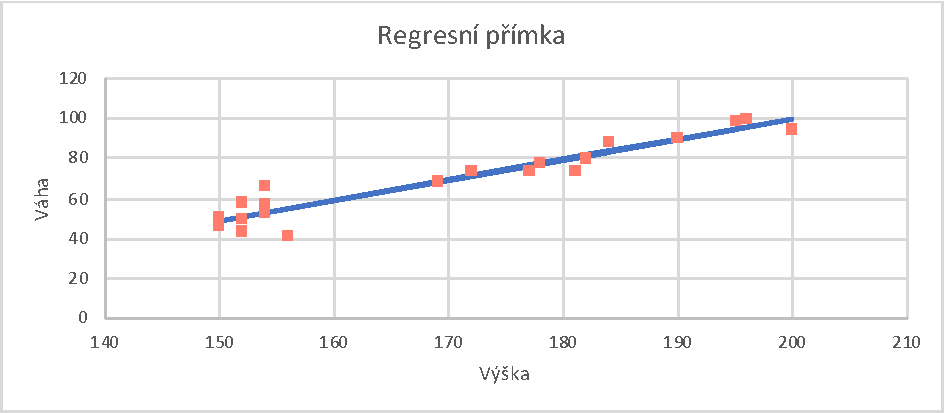
\includegraphics[width=.7 \linewidth]{img/2-c-3-reg-prim.pdf}
	\end{figure}

	\begin{figure}[H]
		\centering
		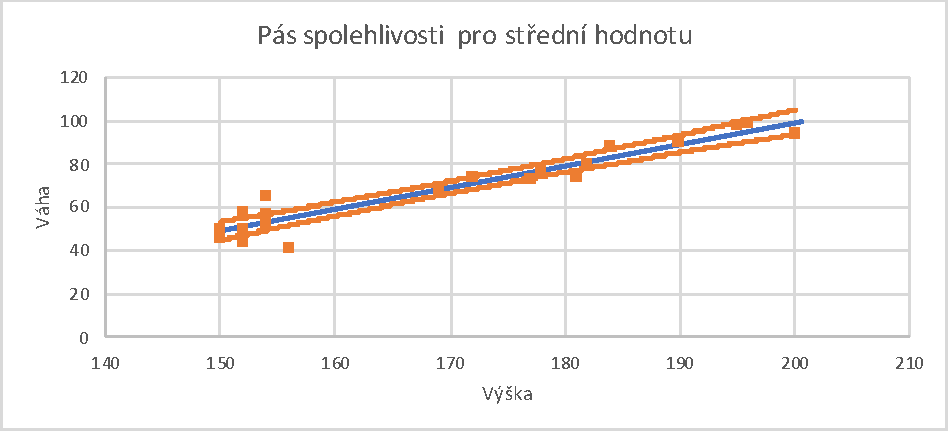
\includegraphics[width=.7 \linewidth]{img/2-c-3-spol-stred.pdf}
	\end{figure}

	\begin{figure}[H]
		\centering
		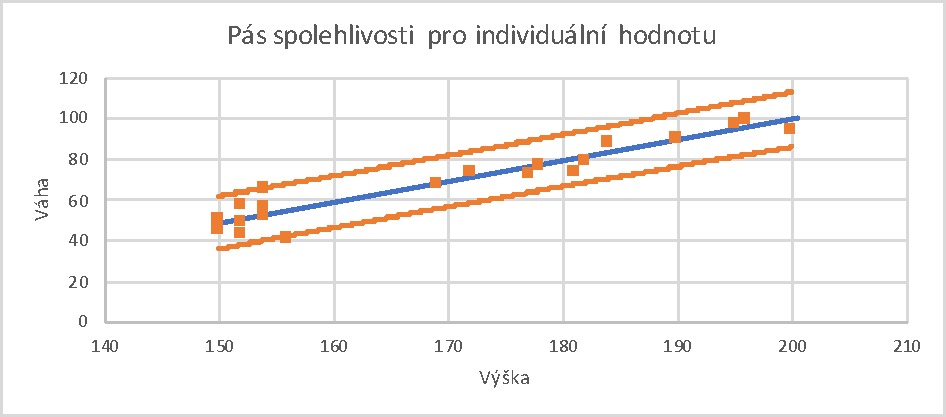
\includegraphics[width=.7 \linewidth]{img/2-c-3-spol-indiv.pdf}
	\end{figure}
\end{document}
